\documentclass[Report.tex]{subfiles}

\newcommand{\baraxis}[8]{
\begin{axis}[
    ybar,
    title={#1},
    width=#5,
    height=#6,
    ymin=#3, ymax=#4,
    bar width=1em,
    legend style={at={#7},anchor=north,legend columns=-1},
    enlarge x limits=0.4,
    x tick label style={align=center,text width=#8},
    symbolic x coords={Logistic Regression, Random Forest, Multi-layer Perceptron},
    xtick=data,
    ylabel={#2}
]
}
% #1 - Number of splits
% #2 - Split number
% #3 - Feature name
% #4 - Column name
% #5 - Column legend name
\newcommand{\plotbar}[5]{
\addplot+[
	discard if not={numSplits}{#1},
	discard if not={split}{#2},
	discard if not={features}{#3},
] table [x=model, y=#4,col sep=comma] {data/19-pair-cv.csv};
\addlegendentry{#5}
}


% #1 - Title
% #2 - Y axis label
% #3 - Legend position
\newcommand{\lineaxis}[5]{
\begin{axis}[
    title={#1},
    width=#3,
    height=#4,
%    ymin=#3, ymax=#4,
%    bar width=1em,
    legend style={at={#5},anchor=north,legend columns=-1},
    enlarge x limits=0.4,
	xlabel={Portion of match},
    ylabel={#2},
]
}


% #1 - ML model
% #2 - Feature name
% #3 - Metric name
% #4 - Legend name
\newcommand{\plotline}[4]{
\addplot+[
	discard if not={numSplits}{5},
	discard if not={model}{#1},
	discard if not={features}{#2}
] table [x=split, y=#3, col sep=comma] {data/19-pair-cv.csv};
\addlegendentry{#4}
}


\begin{document}



\section{Same player identification}\label{sec:pair-classification}
This sections describes the experiments and analysis of the second question: \textit{Given two matches of Dota 2, is it the same player playing on this hero?}

As the question has changed, some parts of the approach for player identification have changed to adapt to the new question. Most notably the the mouse movement features were transformed in order to satisfy the need to have two matches as input instead of just one. 

\subsection{Approach}
%There was a subtle issue with the way the binary classification problem was framed in regards to classifying individual games. This led to high accuracies even with only using mouse movement features, as seen in section \ref{sbsec:game-classification}. The issue had to do with the generality of the model. The models were only trained on a relatively small, fixed set of players, making the problem easier to solve as the models only have to learn the behaviour from the players in the set, which does not apply(TODO) to the general Dota 2 playerbase. Furthermore, the classification is only trained on one particular playing and requires the model to be retrained to be able to predict behaviour of another player. This could be extended into a multi-class problem, but it would still be fixed to the small set of players used in training. This leads to the next machine learning approach of \textit{pair} classification.
%In the next and final approach, deals with this issue by framing the player prediction problem in a different way. Rather than ask \textit{Given a game, which player does it belong to?} the problem is framed as \textit{Given a pair of games, do both games belong to the same player?}
% TODO this leads to low testing accuracies?
% TODO results on a lot more players leads to worse accuracy

The goal of this approach was to be able to train on a large mix of players and games, to learn on features of both matches, and predict if it is the same player, especially if none of the players have been seen by the model before. Instead of learning to match behaviour to specific players, the idea becomes learning the pattern or differences in behaviour between two different players. 

In order to train on pairs of matches together, the input features had to be altered to fit as single data points. In the previous experiment, each match was evaluated separately, so every single mouse action in a game could be used and combined, as explained in section \ref{sec:game-approach}. However, in this pair approach, two matches must be used together as the input to a model. Matches in general are of different lengths, which causes the number of mouse actions to be different for every game. Further, the method of generating each mouse movement means even games of the exact same length will not have the same number of actions. The varying number of mouse actions prevents a straightforward use of them as input to a machine learning model. Instead, statistics such as the mean, standard deviation and range must be used. The statistics are calculated for each mouse movement feature over the entire match. For example, the horizontal velocity of a mouse action creates four features, the mean, standard deviation, minimum and maximum horizontal velocity of each \textit{individual} mouse action. There are numerous mouse actions in every match so further statistics of the four statistical features were created, giving new features such as the mean of the mean horizontal velocities. 

\begin{table}[H]
\centering
\begin{tabular}{| c | c | c | c |}
\hline
\textbf{Original property} & \textbf{Original features} & \textbf{New features} & \textbf{Number of features} \\ \hline
Angle of movement & \multirow{9}{3cm}{Minimum, maximum, mean, standard deviation} & \multirow{11}{3cm}{Minimum, 25\%, 50\%, 75\%, maximum, mean, standard deviation} & \multirow{9}{*}{$ 9 \times 4 \times 7 = 252 $} \\ \cline{1-1}
Curvature &  &  &  \\ \cline{1-1}
Rate of change of curvature &  &  &  \\ \cline{1-1}
Horizontal velocity &  &  &  \\ \cline{1-1}
Vertical velocity &  &  &  \\ \cline{1-1}
Velocity &  &  &  \\ \cline{1-1}
Acceleration &  &  &  \\ \cline{1-1}
Jerk &  &  &  \\\cline{1-1}
Angular velocity & & & \\ \cline{1-2} \cline{4-4}
Game ticks to command & \multirow{2}{*}{Single value} & & \multirow{2}{*}{$ 2  \times 7 = 14 $} \\ \cline{1-1}
Distance to command & & & \\ \hline
\end{tabular}
\caption{New features created after pre-processing mouse movement features for pair classification.}
\end{table}

Clearly, this approach has many drawbacks. The most obvious is the loss of data from taking averages of averages, as the thousands of mouse actions are reduced to only a small number of statistics. To alleviate this issue as much as possible, the matches can be split into a few portions where each portion has its own statistics. For example, a match can be split into thirds where each third has its own mean and standard deviation for each mouse movement feature. Splitting a game this way not only decreases the data loss due to averaging, but enables each portion to be evaluated individually, to see whether any section of a game is more indicative and predictive of player behaviour compared to another section. The drawback with splitting matches like this was the large number of features that were created, leading to the curse of dimensionality and excessive computational requirements in extreme cases. Continuing with the horizontal velocity example, TODO

\subsection{Experimental design}
The experimental design for these experiments follow largely from the design described in section \ref{sec:game-experimental} with a few key differences:
\begin{itemize}
\item For mouse movement and game statistic features, each pair of matches could be split into different slices. This creates more features when used together, as a match split into two slices will have double the features, one set for each half of the match. This also allowed for comparisons to be made for each slice, to see if any portion of a match is more predictive than another. 
\item A modified dataset was created for this set of experiments. The dataset was created in order to prevent data leakage, as the original contained one player which appeared in both the training and testing sets, which made sense in the previous problem. The number of data points in the new modified dataset changed due to the nature of the inputs for each problem. Here, the new dataset was created by taking a combination of every pair of matches, so many more samples can be created with fewer matches. Moreover, no single player belonged to a majority of matches, to prevent models becoming biased towards learning only a particular player's behaviour.

%TODO data changed, not two datasets
%\textbf{Dataset 1} (same as in section \ref{sec:game-classification}) TODO %games (hero id 15) \\
%\textbf{Dataset 2}: m games
\end{itemize}

%In additional to the second dataset, more datasets using different heroes were created in order to give a strong comparison of the best model and features found and testing them on new datasets of different heroes. TODO. 

\subsection{Mouse movement features}
%\newcommand{\plotbarmouse11}[2]{
%\plotbar{1}{1}{mouse}{#1}{#2}
%}

TODO mouse movement with different num split

\begin{figure}[H]
\centering
\begin{tikzpicture}
\baraxis{\textbf{Classification with mouse movement features}}{Metric rate}{0.3}{1.03}{9cm}{5cm}{(0.5,-0.45)}{1.7cm}

\plotbar{1}{1}{mouse}{accuracy}{Accuracy}
\plotbar{1}{1}{mouse}{precision}{Precision}
\plotbar{1}{1}{mouse}{recall}{Recall}

\end{axis}
\end{tikzpicture}
\caption{Accuracy, precision and recall of using mouse movement features only when classifying a pair of matches.}
\end{figure}

Looking at mouse movement features only, it can be seen the the logistic regression model performs poorly compared to the other two models. There are two likely explanations for this. The first, is because logistic regression typically assumes some form of linear relationship between the input and output. As the mouse movement features were not transformed in such a way to better uncover a linear relationship to the output, the non-linear based algorithms of random forest and multi-layer perceptron were better able to distinguish and predict whether the two input matches were from the same player. The second reason why logistic regression may have performed poorly is due to the increased number of features relative to the number of data points available in training. In a comparison of logistic regression to other classifiers, Yoo et al. \cite{lr-vs-rf} demonstrated that logistic regression performed poorly when the number of features was greater than the number of sample data points. That was not the case here, as there were 268 features and a few thousand data points, but perhaps the ratio of features to data points played a role. It is difficult to pinpoint the exact reason, and although further analysis of the other features hints towards the first reason, there are many variables in play which make direct comparisons difficult. 

In a rudimentary comparison to the previous experiment, the results were weaker across the board here. No metric got over 80\% where both logistic regression and multi-layer perceptron models got over 80\% for just mouse movement. This could be attributed to two causes, the loss of data from averaging and the increased difficulty of the problem. The difference in the two datasets makes the comparison difficult, as this dataset creates more data points and has a more diverse number of players. 

% It shall be shown when investigating the other features that the loss of data from averaging was not the root cause. The other features such as itemisation did not have the drawback of averaging but similarly performed worse compared to the previous experiment. 
\begin{figure}[H]
\begin{subfigure}{1\textwidth}
\centering
\begin{tikzpicture}
\baraxis{\textbf{Accuracy of different slices}}{Accuracy rate}{0.3}{1}{9cm}{5cm}{(0.5,-0.45)}{1.7cm}

\plotbar{1}{1}{mouse}{accuracy}{1 slice}
\plotbar{2}{2}{mouse}{accuracy}{2 slices}
\plotbar{3}{3}{mouse}{accuracy}{3 slices}
\plotbar{5}{5}{mouse}{accuracy}{5 slices}

\end{axis}
\end{tikzpicture}
\end{subfigure}

\begin{subfigure}{0.45\textwidth}
\centering
\begin{tikzpicture}[scale=0.75]
\baraxis{\textbf{Precision of different slices}}{Precision rate}{0.3}{1}{9cm}{5cm}{(0.5,-0.45)}{1.7cm}

\plotbar{1}{1}{mouse}{precision}{1 slice}
\plotbar{2}{2}{mouse}{precision}{2 slices}
\plotbar{3}{3}{mouse}{precision}{3 slices}
\plotbar{5}{5}{mouse}{precision}{5 slices}
\legend{};
\end{axis}
\end{tikzpicture}
\end{subfigure}
\hspace{\fill}
\begin{subfigure}{0.45\textwidth}
\centering
\begin{tikzpicture}[scale=0.75]
\baraxis{\textbf{Recall of different slices}}{Recall rate}{0.3}{1}{9cm}{5cm}{(0.5,-0.45)}{1.7cm}

\plotbar{1}{1}{mouse}{recall}{1 slice}
\plotbar{2}{2}{mouse}{recall}{2 slices}
\plotbar{3}{3}{mouse}{recall}{3 slices}
\plotbar{5}{5}{mouse}{recall}{5 slices}
\legend{};
\end{axis}
\end{tikzpicture}
\end{subfigure}
\caption{Metric scores with mouse movement features when a match is split into a different number of portions and they are used together. Note that more slices means a greater number of features, as the featureset is repeated for each slice.}
\end{figure}

When splitting a match into multiple portions and using all portions together in training, the poor performance of logistic regression can again be seen clearly underperforming compared to the other two models. However, a key point of interest is how there is no significant decline in accuracy as the number of splits increases, which one would expect if Yoo et al.'s \cite{lr-vs-rf} findings were to be confirmed, as the difference between 1 split and 5 splits is five times the number of features. The accuracy does fall for 2 splits, but grows again for 3 and 5 splits. This suggests a more complicated reason than simply logistic regression performing poorly because the number of features was too large, likely showing the linear model reaching it's limitations. 

% random forest getting less accuracy with more splits, too many features adds too much noise?

Finally, each individual slice of a match was tested TODO

\begin{figure}[H]
\centering
\begin{tikzpicture}
\lineaxis{Accuracy for different portions of a match}{Accuracy rate}{12cm}{6cm}{(0.5,-0.25)}

\plotline{Logistic Regression}{mouse}{accuracy}{Logistic Regression}
\plotline{Random Forest}{mouse}{accuracy}{Random Forest}
\plotline{Multi-layer Perceptron}{mouse}{accuracy}{Multi-layer Perceptron}

\end{axis}
\end{tikzpicture}
\caption{Metric scores with mouse movement features on individual portions of a match. }
\end{figure}

\subsection{Game statistic features}
Next are the game statistic features. A slightly different trend can be seen compared to the mouse movement features. Logistic regression continues to perform poorly, but the multi-layer perceptron model interestingly has very high recall but low accuracy and precision. This was exactly the same pattern observed when looking at single matches in section \ref{sbsec:game-classification}. This is very interesting as this pattern does not occur in any other combination of features or models. 

% More on same pattern TODO

\begin{figure}[H]
\centering
\begin{tikzpicture}
\baraxis{\textbf{Metrics for classifying pairs of games with game statistic features}}{Metric rate}{0.3}{1.03}{9cm}{6cm}{(0.5,-0.35)}{1.7cm}

\plotbar{1}{1}{stats}{accuracy}{Accuracy}
\plotbar{1}{1}{stats}{precision}{Precision}
\plotbar{1}{1}{stats}{recall}{Recall}

\end{axis}
\end{tikzpicture}
\caption{Accuracy, precision and recall rates using only game statistics such as gold and XP per minute when classifying a pair of matches.}
\end{figure}

The random forest classifier gave the best results with just game statistics by a large margin. This was somewhat expected, as it also performed the best in the previous experiment. It is interesting that the performance was able to be translated to this experiment very well. This shows a strong correlation between in game statistics and player prediction, both in identifying a particular player and in identifying the difference between two players. 

\begin{figure}[H]
\vspace{-2cm}
\begin{subfigure}{1\textwidth}
\image{0.9\textwidth}{imgs/correlation-stats0.png}{Correlation matrix for pairs by different players}
\end{subfigure}

\begin{subfigure}{1\textwidth}
\image{0.9\textwidth}{imgs/correlation-stats1.png}{Correlation matrix for pairs by the same players}
\end{subfigure}
\caption{Correlation matrices showing the statistics for one match of a pair against the other.}
\label{fig:stats-correlation}
\end{figure}

The correlation between the statistics of one match compared to the statistics of the other match in a pair can help give insight into which statistics are more impactful. Figure \ref{fig:stats-correlation} shows the correlation matrices between pairs by different players and pairs by the same players. The differences between the two matrices again show much higher correlation for pairs where both matches were by the same player. A small number of statistics are seen to be stronger indicators than others. First, the kills, deaths and assists (KDA) do not look well correlated. This was speculated earlier, as the KDA of players vary often in a small range. The gold and XP statistics are also better correlated between two matches by the same player when looking at per minute statistics instead of the absolute gold and XP earned by the end of a match. 

There are a few key points to notice for the gold and XP per minute statistics. The CS, denies, gold per minute, XP per minute and cs per minute scores are well correlated to each other even across different matches, as long as the player was the same. It would be expected for these numbers to be correlated in the same match, as creeps directly affect the gold and XP gained by heroes. However, seeing the statistics continue this trend across different matches suggest they are also tied to specific player behaviour. The same pattern can be seen for movement commands, and to a lesser extent the attack and spell cast commands. This is very interesting, and suggests using the statistics together gives better results that compared each individually across a pair. 

Finally, it should be noted that the correlation matrix for pairs of matches by the same players is mirrored across the diagonal. This is a results of the combination step, where matches are combined into pairs of \textit{\{match0, match1\}} and \textit{\{match1,match0\}} and should not be taken as a meaningful results.


Due to the way the \texttt{clarity} parser functions by running through matches chronologically, and a bug which prevents the library from seeking directly to a time or tick in a match, splitting up a match into equally sized portions on the go was not possible and so, detailed data about game statistics on different sections of a match could not be gathered.  
%MORE reasoning TODO

\subsection{Itemisation features}

For itemisation features, each encoding method can be compared. On the whole, using only boots by themselves was the best indicator for random forest and multi-layer perceptron, while the item differences were best for the logistic regression model. Once again, logistic regression did not have good results compared to the random forest and multi-class perceptron models. The only exception is the item difference method of encoding, where it was able to get higher accuracies than the random forest and multi-layer perceptron models. This is a bit of an anomaly, as the trend so far suggests logistic regression is not suitable for this classification task.  


\begin{figure}[H]
\centering
\centering
\begin{tikzpicture}
\baraxis{\textbf{Accuracy with game itemisation features}}{Accuracy rate}{0.4}{1}{15cm}{4.5cm}{(0.5,-0.35)}{2cm}

\plotbar{1}{1}{items-hashed}{accuracy}{Hashed items}
\plotbar{1}{1}{items-onehot}{accuracy}{One-hot}
\plotbar{1}{1}{items-starting}{accuracy}{Starting items}
\plotbar{1}{1}{items-select}{accuracy}{Boots only}
\plotbar{1}{1}{items-diff}{accuracy}{Item differences}
\legend{};
\end{axis}
\end{tikzpicture}

\begin{tikzpicture}
\baraxis{\textbf{Precision with game itemisation features}}{Precision rate}{0.4}{1}{15cm}{4.5cm}{(0.5,-0.35)}{2cm}

\plotbar{1}{1}{items-hashed}{precision}{Hashed items}
\plotbar{1}{1}{items-onehot}{precision}{One-hot}
\plotbar{1}{1}{items-starting}{precision}{Starting items}
\plotbar{1}{1}{items-select}{precision}{Boots only}
\plotbar{1}{1}{items-diff}{precision}{Item differences}
\legend{}; % hide legend

\end{axis}
\end{tikzpicture}

\begin{tikzpicture}
\baraxis{\textbf{Recall with game itemisation features}}{Recall rate}{0.4}{1}{15cm}{4.5cm}{(0.5,-0.38)}{2cm}

\plotbar{1}{1}{items-hashed}{recall}{Hashed items}
\plotbar{1}{1}{items-onehot}{recall}{One-hot}
\plotbar{1}{1}{items-starting}{recall}{Starting items}
\plotbar{1}{1}{items-select}{recall}{Boots only}
\plotbar{1}{1}{items-diff}{recall}{Item differences}


\end{axis}
\end{tikzpicture}
\caption{Accuracy, precision and recall for different game itemisation encoding methods.}
\end{figure}

There are a few surprising results for the different encoding methods. Firstly, the one-hot encoding of all items performed very similarly to the one-hot encoding of only starting items. This was surprising because the one-hot encoding of all items contained 250 more items than the starting items, which translates to 1500 more binary features. Furthermore, the one-hot encoding of all items sampled the hero inventory twice, once at the start and once at the end of a match. This would again double the number of features compared to looking at only the starting items. 

%TODO check end items being used properly

\subsection{Combined features}

\subsubsection{Comparison of feature individually}

\begin{figure}[H]
\newcommand{\comparisonaxis}[2]{
\begin{axis}[
	title={\textbf{#1}},
	ylabel={#2},
	ybar,
	bar width=1.5em,
	width=15cm,
	height=4cm,
	legend style={at={(0.5,-0.35)},anchor=north,/tikz/every even column/.append style={column sep=0.5cm}},
	xtick=data,
	enlarge x limits=0.25,
	ymin=0.4, ymax=1,
	symbolic x coords={Logistic Regression, Random Forest, Multi-layer Perceptron},
    x tick label style={align=center,text width=2.5cm},
]
}
\centering
\begin{tikzpicture}
\comparisonaxis{Accuracy of features individually}{Accuracy rate}

\plotbar{1}{1}{mouse}{accuracy}{Mouse movement only}
\plotbar{1}{1}{stats}{accuracy}{Game statistics only}
\plotbar{1}{1}{items-onehot}{accuracy}{All items with one-hot encoding}
\plotbar{1}{1}{items-starting}{accuracy}{Starting items only}
\legend{};
\end{axis}
\end{tikzpicture}

\begin{tikzpicture}
\comparisonaxis{Precision of features individually}{Precision rate}

\plotbar{1}{1}{mouse}{precision}{Mouse movement only}
\plotbar{1}{1}{stats}{precision}{Game statistics only}
\plotbar{1}{1}{items-onehot}{precision}{All items with one-hot encoding}
\plotbar{1}{1}{items-starting}{precision}{Starting items only}
\legend{};
\end{axis}
\end{tikzpicture}

\begin{tikzpicture}
\comparisonaxis{Recall of features individually}{Recall rate}

\plotbar{1}{1}{mouse}{recall}{Mouse movement only}
\plotbar{1}{1}{stats}{recall}{Game statistics only}
\plotbar{1}{1}{items-onehot}{recall}{All items with one-hot encoding}
\plotbar{1}{1}{items-starting}{recall}{Starting items only}

\end{axis}
\end{tikzpicture}
\caption{Accuracy for pair classification with different features and models.}
\end{figure}


It can be concluded quite definitively from analysing the features individually that logistic regression was not well suited to this classification problem. In every feature, logistic regression struggled to get a 50\% classification rate, with only the boots only feature getting a 59\% correct classification. As such, there is a clear difference in the complexity of the classification problem compared to the previous experiment, where logistic regression was able to obtain strong results. It is also unlikely that Yoo et al.'s explanation of poor logistic regression performance with a large number of features \cite{lr-vs-rf} applies here, as the game statistic features had a small number of features while mouse movement had a large number of features. 

There are a few model and feature combinations that stand out with the best individual performance. Random forest in general was able to obtain high accuracies with all different features. The neural network had comparable results for the itemsation features, but not for the mouse movement or statistic features. This is interesting because the mouse movement and statistic features were the best performing features for the random forest classifier. This suggests there is no stand out best feature to determine if two matches come from the same player, but rather, different models are able to apply the different features with varying degrees of success. A similar conclusion was reached by Liu et al. \cite{starcraft-identification} for player identification in Starcraft 2. 

\subsubsection{Combining best features together}
Finally, the individual featuresets are combined together to see if any combination of them may give improved predictive performance. Data for logistic regression regression is not presented as there was next to no performance change for all the different combinations of featuresets, further confirming the linear model as unsuitable for this task. 

\begin{figure}[H]
\newcommand{\combinedbar}[5]{
\addplot+[
	discard if not={numSplits}{#1},
	discard if not={split}{#2},
	discard if not={features}{#3},
	%discard if={model}{Logistic Regression}
] table [x=model, y=#4,col sep=comma] {data/19-pair-cv.csv};
\addlegendentry{#5}
}
\centering
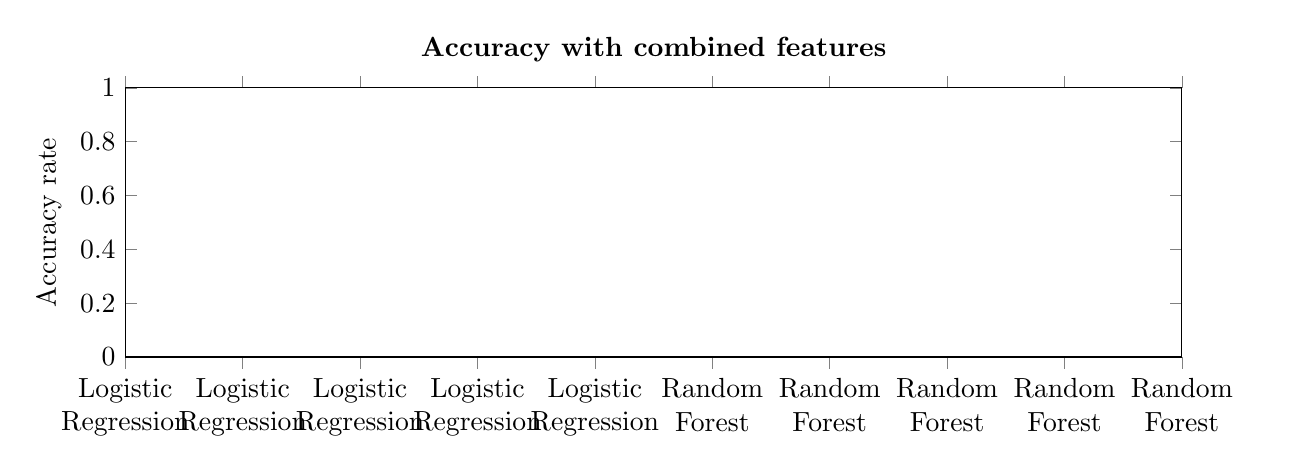
\begin{tikzpicture}
\begin{axis}[
    ybar,
    title={\textbf{Accuracy with combined features}},
    width=15cm,
    height=5cm,
    ymin=0.4, ymax=1,
    bar width=1.5em,
    legend style={at={(0.5,-0.35)},anchor=north,legend columns=-1},
    enlarge x limits=0.4,
    x tick label style={align=center,text width=2cm},
    symbolic x coords={Logistic Regression, Random Forest, Multi-layer Perceptron},
    xtick=data,
    ylabel={Accuracy rate},
    cycle list name=exotic,
    every axis plot/.append style={fill,draw=none,no markers}% <- added
]
%\baraxis{\textbf{Accuracy with combined features}}{Accuracy rate}{0.3}{1.03}{15cm}{6cm}{(0.5,-0.35)}

\combinedbar{1}{1}{mouse-stats}{accuracy}{Mouse-stats}
\combinedbar{1}{1}{mouse-items-onehot}{accuracy}{Mouse-items-onehot}
\combinedbar{1}{1}{mouse-items-select}{accuracy}{Mouse-items-select}
\combinedbar{1}{1}{mouse-stats-items-diff}{accuracy}{Mouse-stats-items-diff}

\end{axis}
\end{tikzpicture}
\end{figure}

\subsection{Different heroes TODO}
% Use same model and features (best ones) , with only hero differ
% hero id 20, 19 and 15
\end{document}

